\chapter{Grundlagen}
\label{chap:grundlagen}

\section{Fortlaufendes Beispiel}
\label{sec:grundlagen:beispiel}

% Beispiel einleiten
Eine einheitliche und fortlaufende Problemstellung soll der Arbeit als Grundlage dienen. Die Problemstellung besteht aus einem Modell und einem Satz von Testdaten. Alle im weiteren Verlauf diskutierten Modellierungsvarianten werden  die Problemstellung umsetzen und die Testdaten modellieren.  

\subsection{Voraussetzungen}
\label{sec:grundlagen:beispiel:voaussetzungen}

Der Schwerpunkt der Modellierung liegt bei der Darstellung von Beziehungen zwischen Entit�ten. Dabei soll die Problemstellung einerseits nicht zu komplex sein, damit sie �berschaubar bleibt. Andererseits soll sie komplex genug sein, um m�glichst alle m�glichen Bezeihungen zwischen Entit�ten abzudecken. 

Die Testdaten sollten so gew�hlt werden, dass idealerweise f�r alle Tests die selben Daten verwendet werden k�nnen. Einheitiche Daten sorgen daf�r, dass sich der Entwickler (verbessern) nicht bei unterschiedlichen Tests in verschiedene Testdaten hineinversetzten muss. Nur in Ausnahmef�llen sollten Tests modifizierte oder eigene Testdaten verwenden.
Um dem Entwickler entgegen zu kommen, sollte der Umfang der Testdaten nicht gr��er sein als erforderlich.

\subsection{Gew�hlte Problemstellung}
\label{sec:grundlagen:beispiel:gewaehlte_problemstellung}
Das gew�hlte Beispiel stellt eine starke Vereinfachung des Pr�fungswesens an Hochschulen dar. Auf eine praxisnahe Umsetzung wird zugunsten der Komplexit�t verzichtet. Es beinhaltet die folgenden vier Entit�ten:

\begin{itemize}
	\item \textbf{Professor}: Ein Professor leitet Lehrveranstaltugnen.
	\item \textbf{Lehrveranstaltung}: Eine Lehrveranstaltng wird von einem Professor geleitet. Es kann zu jeder Lehrveranstaltung eine Pr�fung geben.
	\item \textbf{Pr�fung}: Eine Pr�fung ist einer Lehrveranstaltung zugeordnet. Au�erdem hat mindestens ein Pofessor Aufsicht.
	\item \textbf{Student}: Studenten k�nnen an Lehrveranstaltungen und an Pr�fungen teilnehmen. Studenten haben au�erdem 
		die M�glichkeit, Tutoren von Lehrveranstaltugen zu sein.
\end{itemize}

Abbildung \ref{img:uml_beispiel} stellt die Problemstellung grafisch dar. Die Abbildung zeigt, dass es keine 1:1-Beziehung gibt. Eine 1:1-Beziehung kann jedoch als Spezialfall einer 1:n-Beziehung angesehen werden.

\begin{figure}[H]
	\centering
	 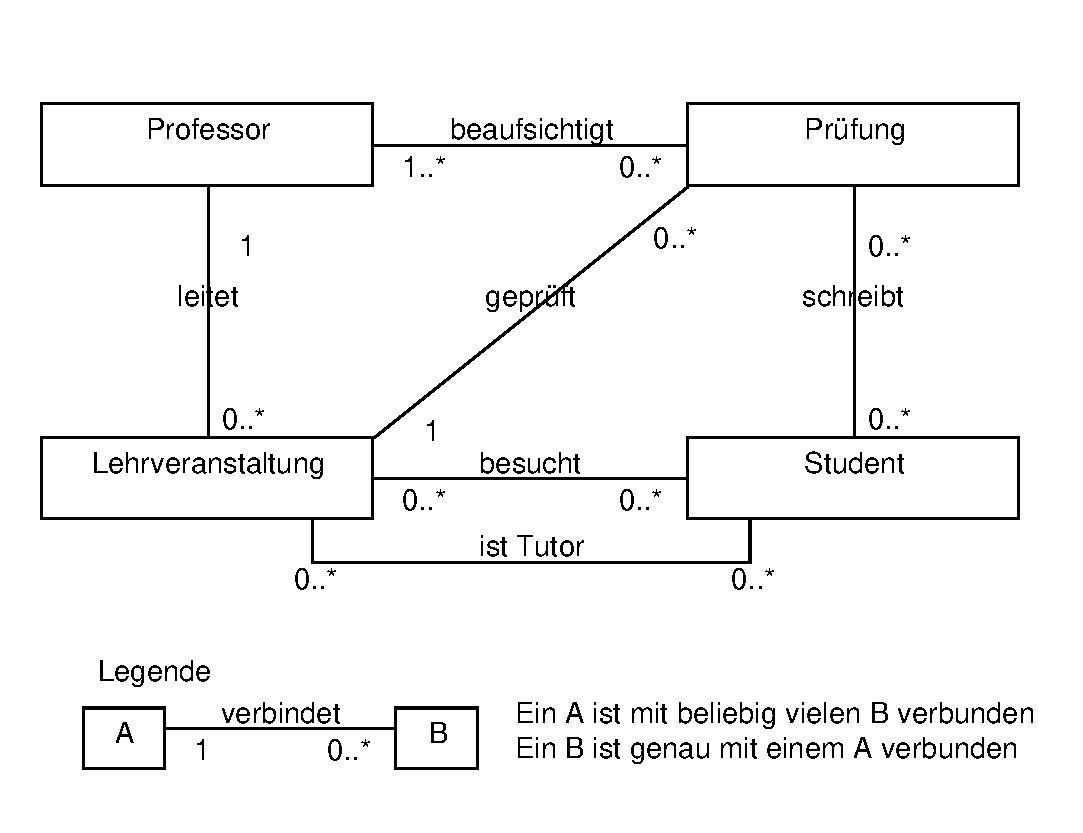
\includegraphics[width=0.8\textwidth]{images/grundlagen/example_hochschule.pdf}
	\caption{UML-Diagramm des fortlaufenden Beispiels}\label{img:uml_beispiel}
\end{figure}

Das entsprechende Datenbankschema sieht folgenderma�en aus:
\begin{figure}[H]
	\centering
	 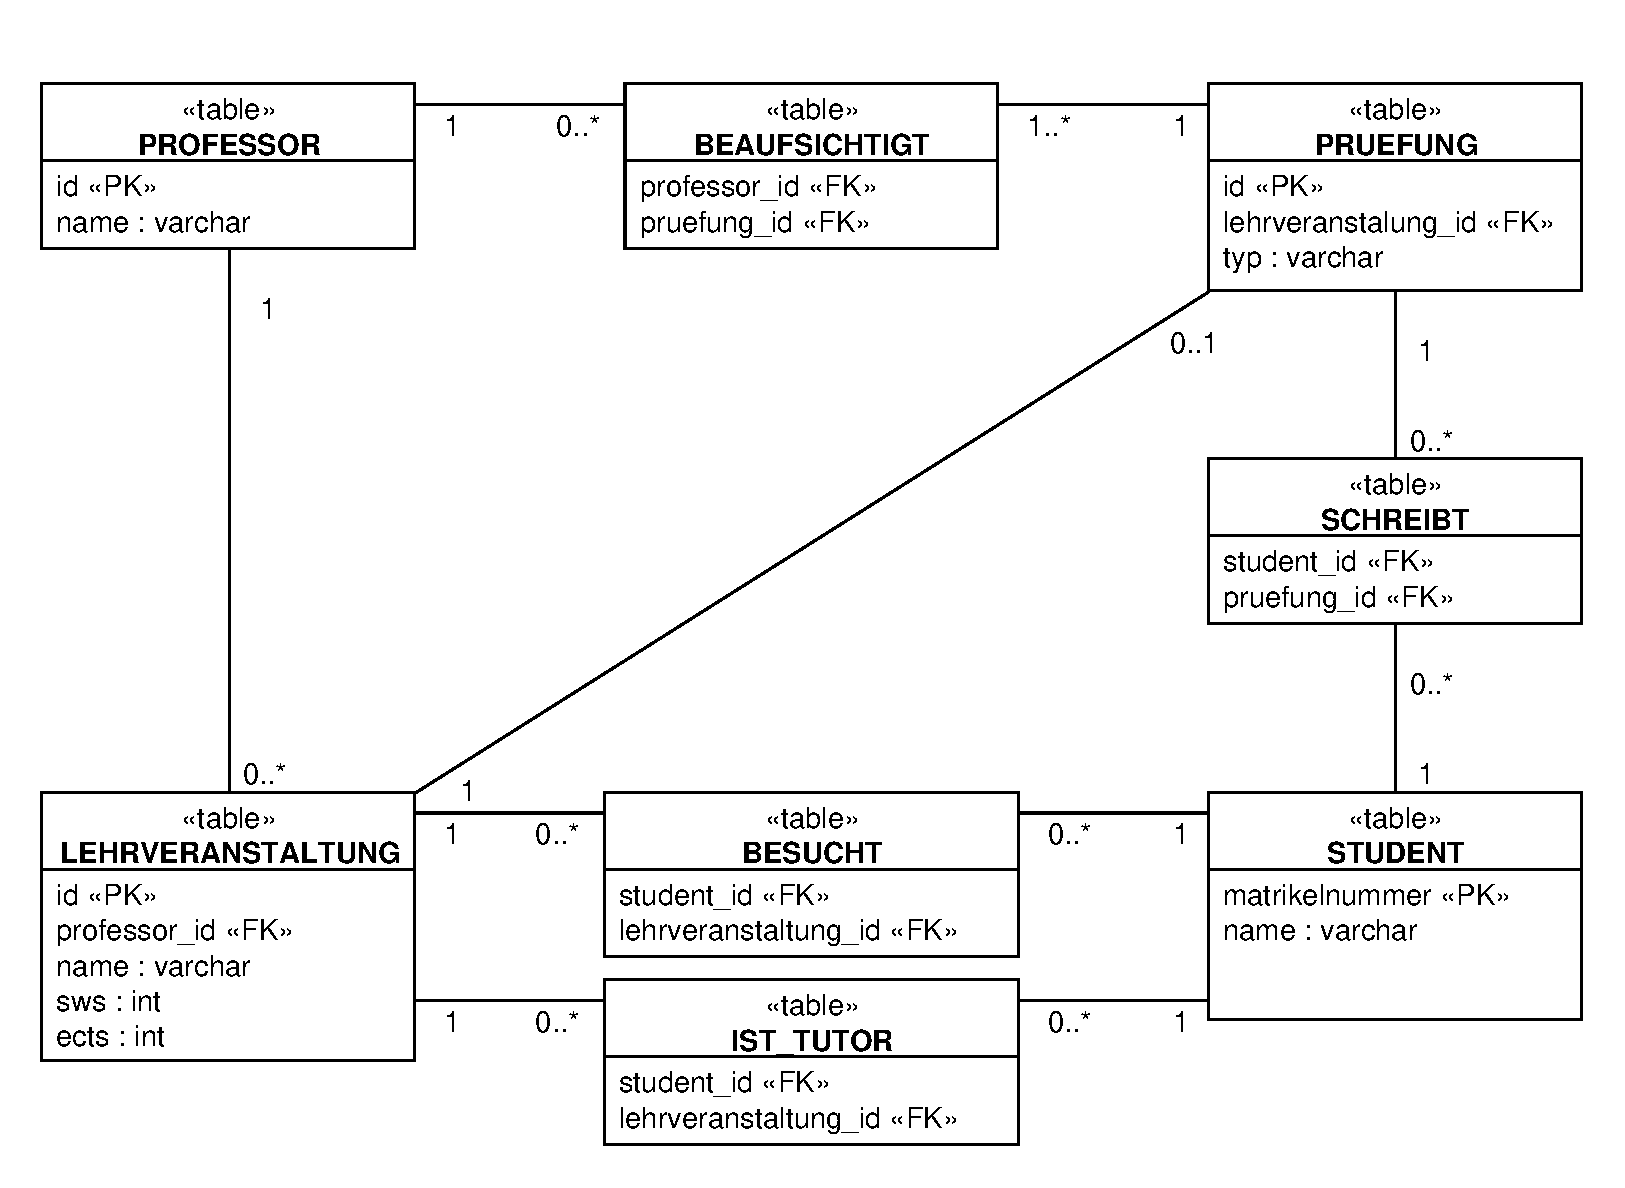
\includegraphics[width=0.95\textwidth]{images/grundlagen/example_hochschule_database.pdf}
	\caption{Datenbank-Diagramm des fortlaufenden Beispiels}\label{img:database_beispiel}
\end{figure}

\subsection{Wahl der Testdaten}
\label{sec:grundlagen:beispiel:testdaten}

Um den einen Kompromiss f�r die Komplexit�t der Testdaten zu finden, werden vier Fragestellungen definiert. Diese Fragen sollen dabei helfen, den Umfang der Testdaten bestimmen zu k�nnen. Die Fragen stellen sich wie folgt dar:

\begin{enumerate}
	\item Welcher Professor unterrichtet die meisten Studenten?
	\item Welcher Student nimmt an den meisten Pr�fungen teil?
	\item Welcher Student ist Tutor und nimmt gleichzeitig an der Pr�fung teil?
	\item Welcher Professor macht die wenigste Aufsicht in Fremdveranstaltungen (Lehrveranstaltungen eines anderen Professors)?
\end{enumerate}



